\providecommand{\main}{..}
\documentclass[\main/main.tex]{subfiles}

\begin{document}
\graphicspath{{img/}{01_intro/img/}}

\chapter{Introduction}

\section{Problem Statement}
Localization has always been in problem throughout history. From the old days when people used to follow the ancient guiding-star navigation until now, a lot of technology has been introduced and finally, Global Positioning System (GPS) has practically solved the problem of outdoor localization. As GPS makes use of satellites, which are located a few thousand miles away from the ground, signals from satellites are obstructed on way from satellites to devices, result in weak signals. Different barriers such as trees and buildings reflecting weak signals also cause multi-path interference. Moreover, the building materials may make it more difficult to perform indoor tracking through GPS. As a result, to provide a GPS-like system for the indoor environment, a lot of studies have been done to develop a full-featured effective and accurate Indoor Positioning System (IPS).
\newline\newline
A navigation system which is made of network devices to locate objects or people with the capability to localize the position of wireless-capable devices within a particular space inside an indoor environment is referred as IPS \cite{survey_on_indoor_wireless_positioning_techniques}. After a great success in adopting with GPS, developing IPS has become a popular research area due to its increasing demand. People want to use indoor positioning systems for various purposes such as security, finding the location of materials and emergency. 
\newline\newline
Many techniques can be used for localization \cite{a_survey_on_localization_for_mobile_wireless_sensor_networks}.Traditionally, different infrastructure such as Wi-Fi, Bluetooth are re-purpose to estimate location for indoor environments. The common approach to estimating distance or location with Wi-Fi and Bluetooth signals is to measure signal strength. The problem with such an approach, of course, is that signal strength is a poor indicator of distance.
\newline\newline
Ultra-wideband (UWB) is a radio technology which makes extremely precise indoor positioning possible. Goods, vehicles and machines can be located with an accuracy of 10-30 centimeters compared with Bluetooth (1-3 meters) or Wi-Fi (5-15 meters). The position determination is carried out by means of a run-time method (Time of Flight, ToF). For this, at least three so-called anchors are required. The time of a flight between anchors and assets is measured by tags attached to the asset. The position is then calculated from such measurements.
\newline\newline
The DW1000 is a fully integrated single-chip Ultra-Wideband (UWB) low-power low-cost transceiver IC compliant to IEEE802.15.4-2011. It can be used in 2-way ranging or TDOA location systems to locate assets to a ranging precision of 10 cm. It also supports data transfer at rates up to 6.8 Mbps \cite{decawave:dw1000_datasheet}.
\newline\newline
The Decawave's DWM1001C module combines the DW1000, a Nordic Semiconductor nRF52832 MCU, and a 3-axis accelerometer. Using this module accelerates the design cycle, reduces development costs, and shortens time to market.
\newline\newline
Decawave also provides a reference solution for the indoor positioning problem. However, this system is closed-source and requires a UWB-capable device in each cell to act as a gateway. Therefore, an extra infrastructure is needed to communicate between gateways. In practice, an IP network is utilized for this purpose which results in more hardware and increases the system cost.
In comparison with the vendor system, this thesis provides a solution to reduce the system cost while brings a similar performance and potentially some IoT services. This thesis makes use of Bluetooth mesh technology to replace the IP network. As the Bluetooth hardware has been pre-implemented in the module, no additional hardware is required.

\section{Thesis Objective}
The main objective of this thesis is to design and implement an indoor localization system using the UWB-based DWM1001C module. In addition, a system based on a Bluetooth mesh network is also built to manage and control the localization system. The mesh network also provides some IoT services for remote control and self-identification.

% \begin{figure}[H]
%     \begin{center}
%         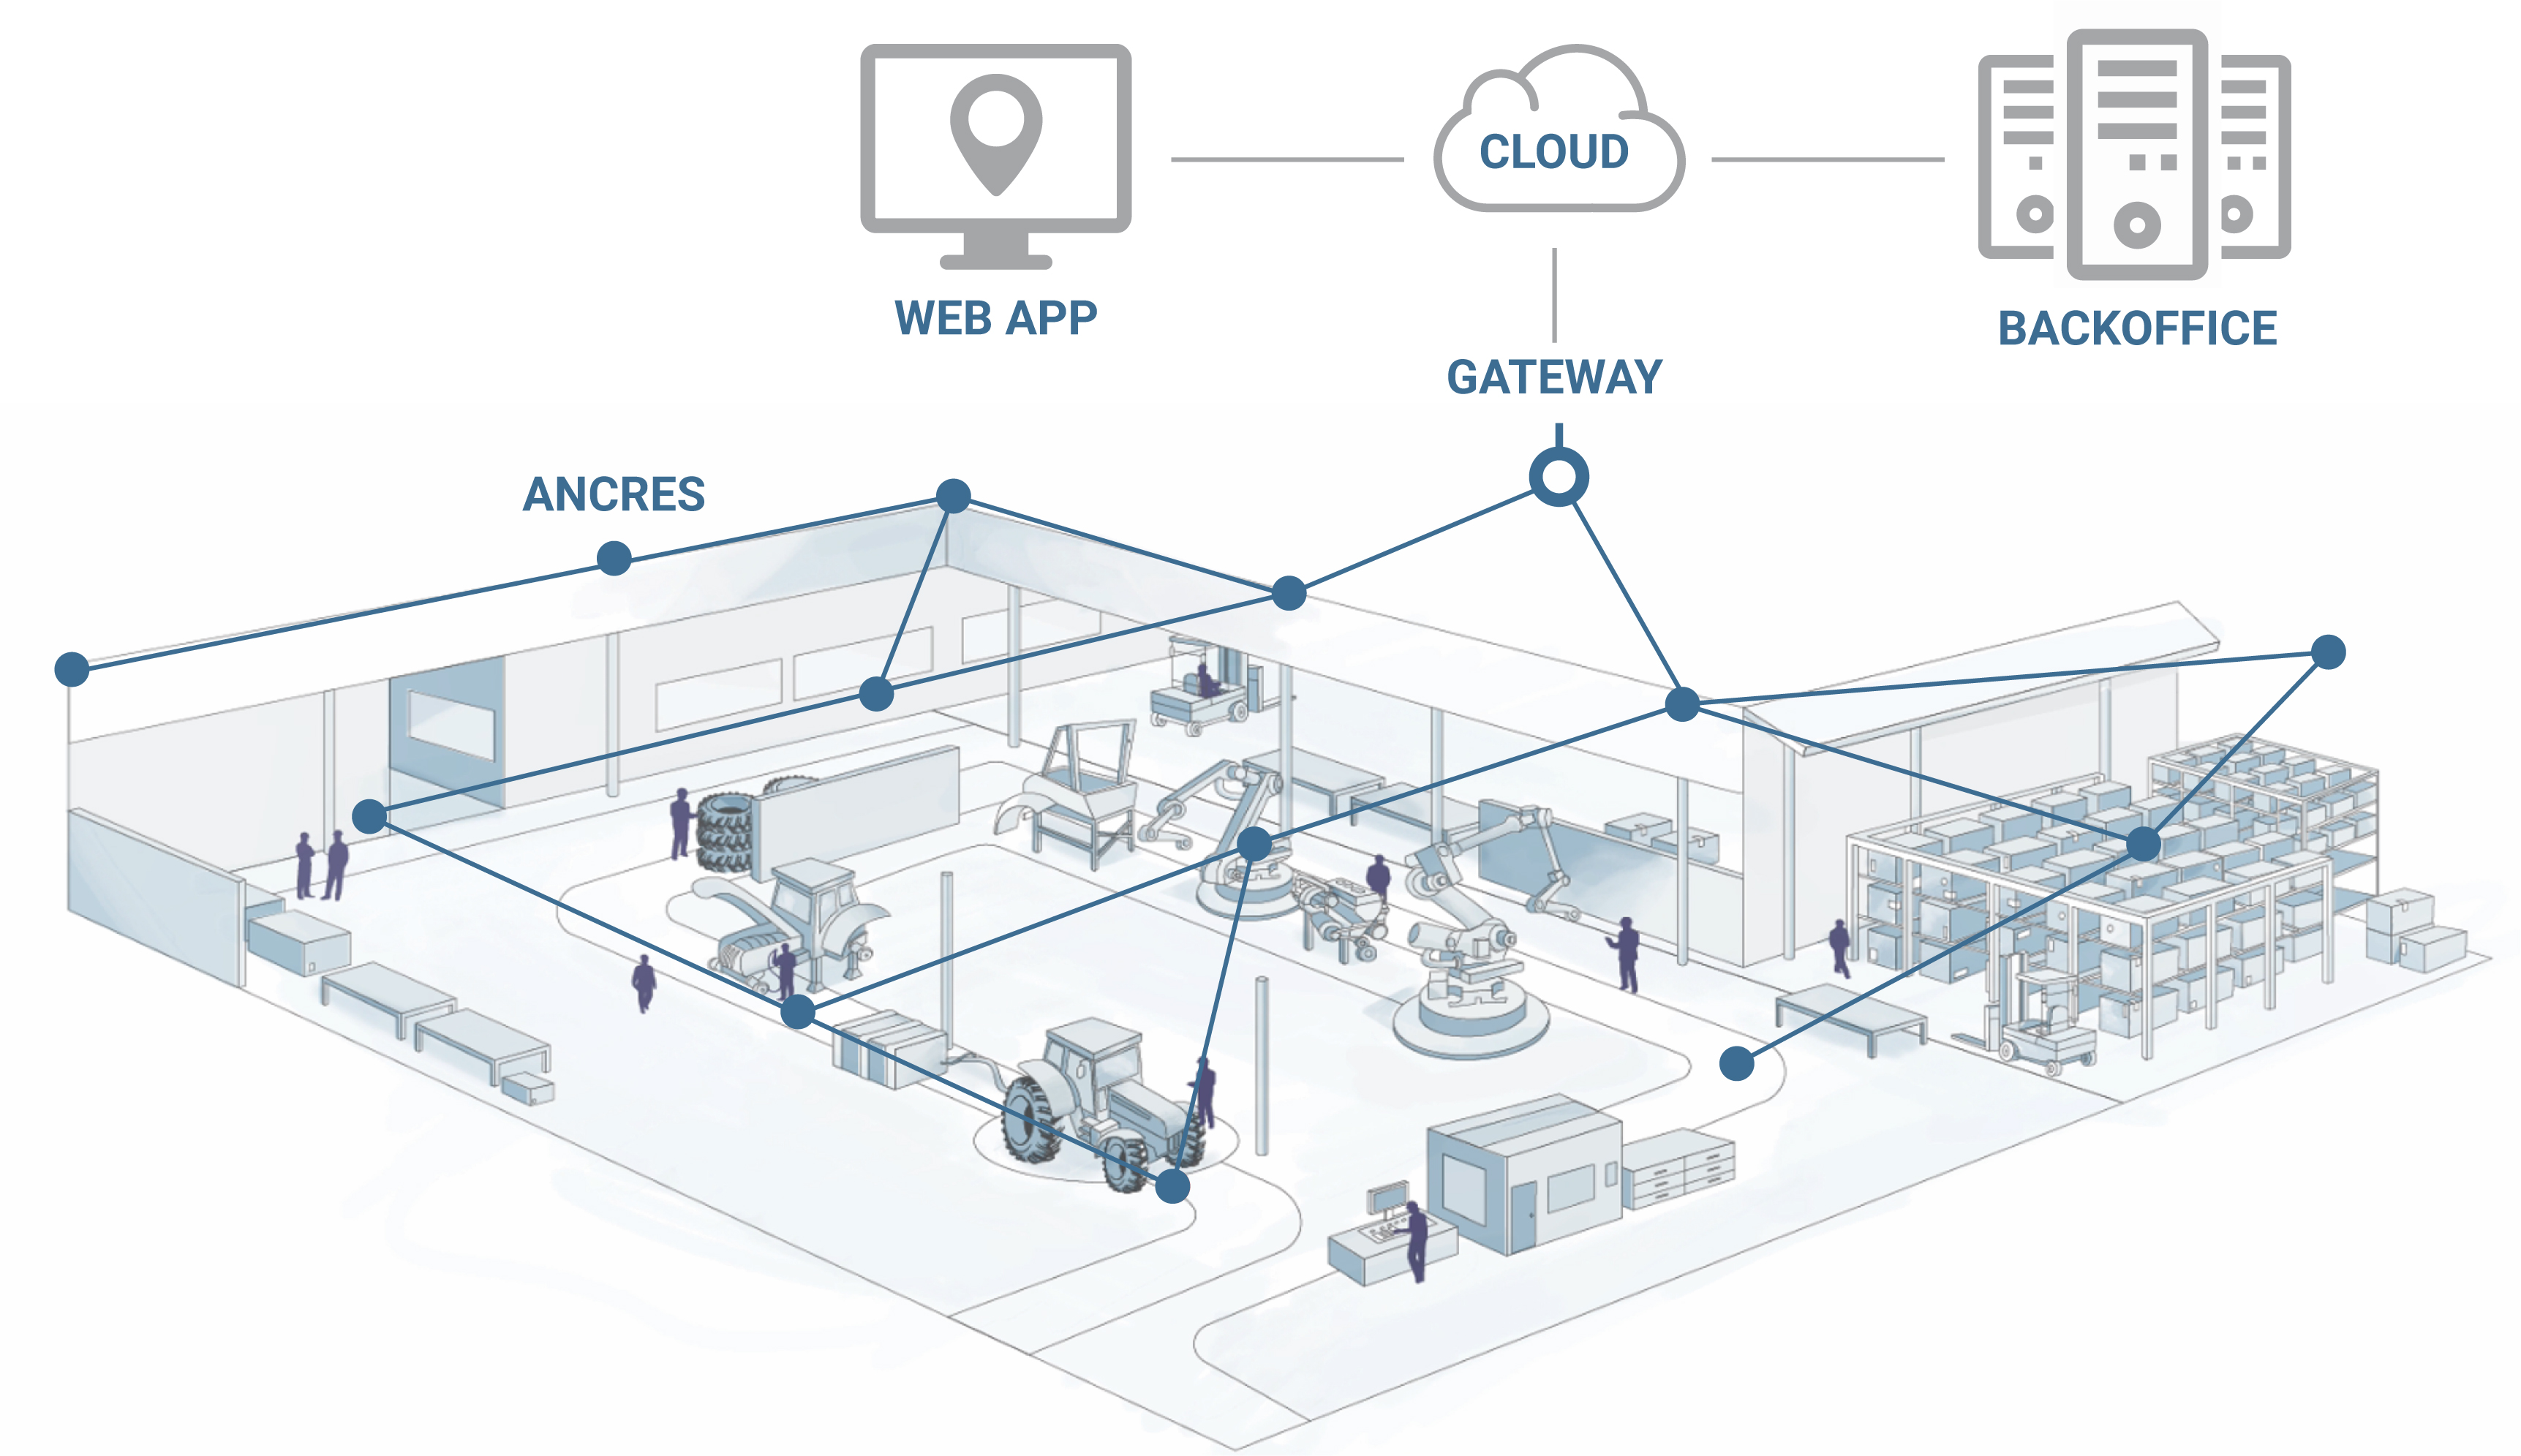
\includegraphics[width=0.9\textwidth]{fonctionnement-technologie-mesh-wirepas.jpg}
%     \end{center}
%     \caption{Indoor location problem}
%     \label{fig:indoor_location}
% \end{figure}

\section{Thesis Structure}
This thesis consists of 9 chapters. In the following, a brief description of each chapter is given.
\begin{itemize}
    \item Chapter 1 is an introduction to the problem of the thesis, the proposed solution, and the objectives of this work.
    \item Chapter 2 is a quick explanation of UWB, its advantages, and regulations. Chapter 2 also discusses the modulation scheme and the IEEE standard for UWB.
    \item Chapter 3 describes some techniques used to estimate the position. This thesis especially focuses on the TWR method for distance measurement and multilateration approach for solving to location.
    \item Chapter 4 discusses the stack implemented in firmware for a TDMA-based ranging system.
    \item Chapter 5 gives a short introduction about Bluetooth mesh and the manner such a network is used in this thesis.
    \item Chapter 6 deals with problems related to the hardware implementation of an anchor.
    \item Chapter 7 introduces the software part used to control and manage both the UWB-based network and the Bluetooth mesh network.
    \item Chapter 8 provides an evaluation result of the proposed system compared with the reference system.
    \item Chapter 9 summarizes the accomplishment and plans for future work.
\end{itemize}
\bib
\end{document}